\section{Resultados}

% LES COPIO LO QUE TENIA EN EL CUADERNO:
% 	Delays en distintos momentos del dia? 
%	Se congestionan los enlaces en horas pico? (ver cuales son las horas pico en cada pais del enlace). 
%	Se utilizan los enlaces si voy a otras paginas cercanas a las que probamos? 
%	Cambian las rutas que se toman a una misma pagina? 
%	Ver tiempos de encolamiento (hacer algun tipo de analisis sobre esto supongo)

%Los datos de los siguientes graficos se midieron utilizando el Traceroute implementado por nosotros. El metodo de medicion fue el siguiente:

***** ACA NO ESTOY SEGURO DE COMO VICKY HIZO LAS MEDICIONES.. POR FAVOR COMPLETAR!! ****

En las figuras \ref{fig:mapa_fin} y \ref{fig:mapa_ing} se muestra una localizacion aproximada de los enlaces transoceánicos utilizados.\\

El primero es un enlace de Estados Unidos (Florida segun IP2Location, Colorado segun IPLigence), a ``Europa'' (segun \url{http://www.geoiptool.com/es/} y \url{www.ipaddresslabs.com}), que detectamos rastreando la ruta hacia \url{www.helsinki.fi} (IP: 128.214.222.4, Finlandia). \\

\begin{itemize}
 \item IP en America: 67.17.106.162
 \item IP en Europa: 213.248.76.189\\
\end{itemize}

\begin{figure}[H]
  \centering
    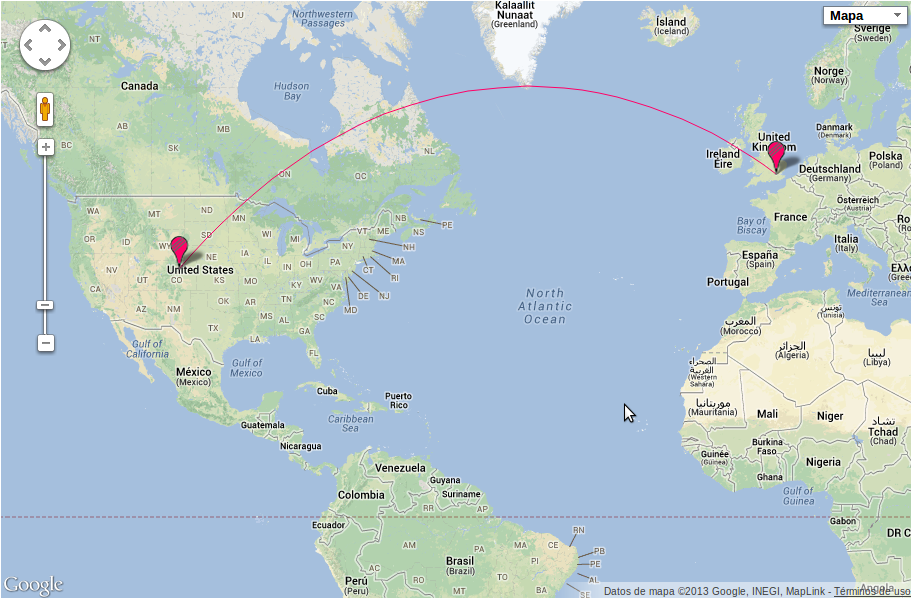
\includegraphics[width=0.9\textwidth]{imgs/finlandia_enlace_1.png}
    \caption{Mapa con la ubicacion aproximada del enlace tomado hacia el host \url{www.helsinki.fi} (Finlandia)}
    \label{fig:mapa_fin}
\end{figure}    

El segundo es un enlace de Estados Unidos (Colorado segun IPligence) a Alemania (segun IPligence), detectado en el camino a \url{www.ox.ac.uk} (IP: 163.1.60.42, Reino Unido).

\begin{itemize}
 \item IP del lado de America: 67.16.139.18
 \item IP del lado de Europa: 141.136.107.37\\
\end{itemize}


\begin{figure}[H]
  \centering
    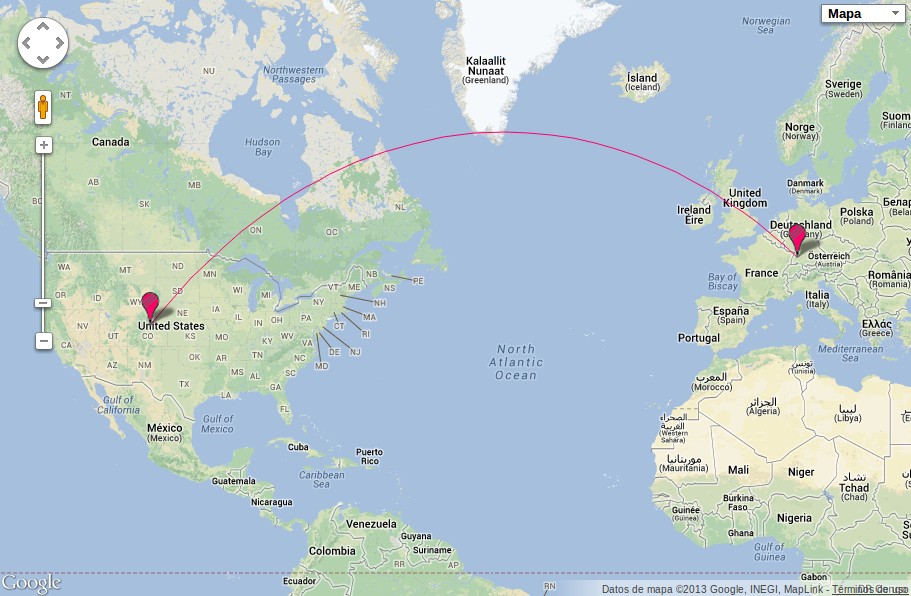
\includegraphics[width=0.9\textwidth]{imgs/inglaterra_enlace_1.png}
    \caption{Mapa con la ubicacion aproximada del enlace tomado hacia el host \url{www.ox.ac.uk} (Reino Unido)}
    \label{fig:mapa_ing}
\end{figure}


\begin{figure}[H]
  \centering
    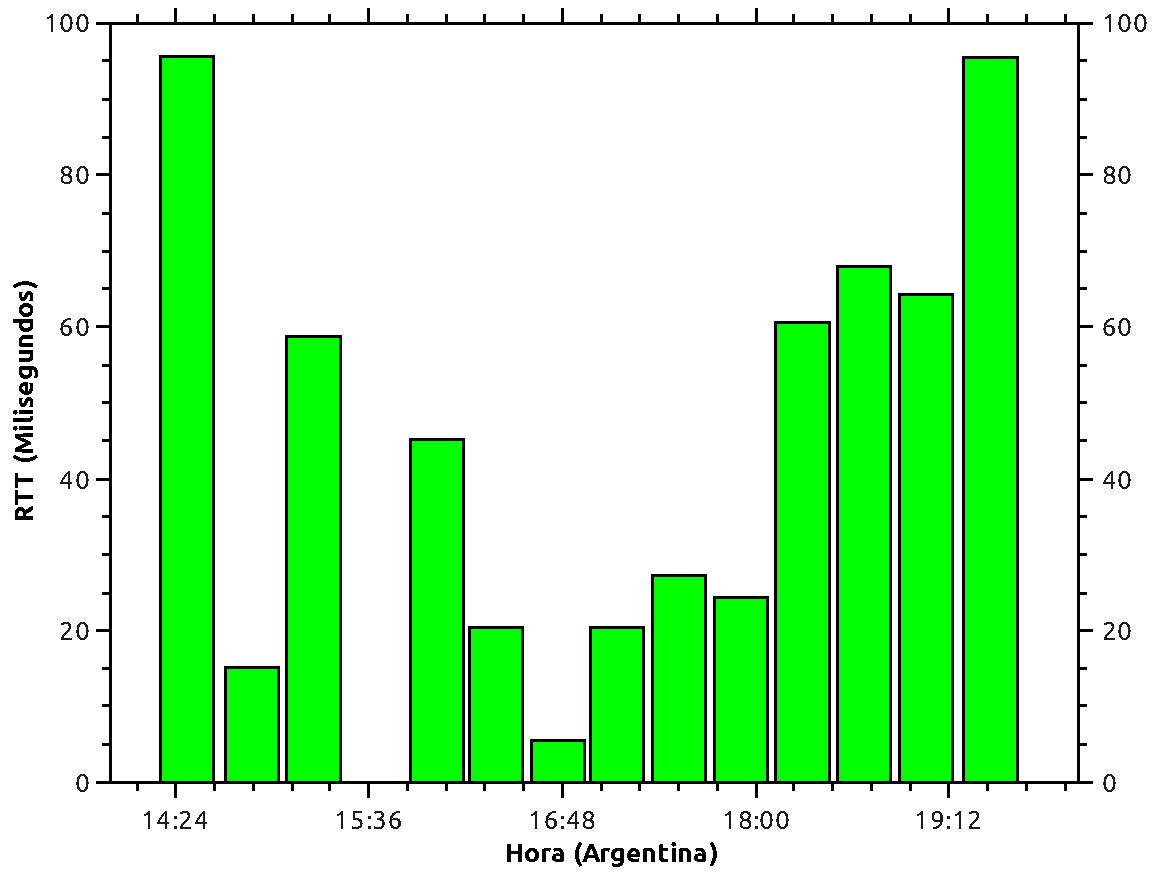
\includegraphics[width=0.9\textwidth]{graficos/rtts_dia_finlandia.pdf}
    \caption{RTTs medidos a lo largo del dia en el enlace EEUU-RU}
    \label{fig:rtts_fin}
\end{figure}

%EEUU : -3
%FINLANDIA: +4

En la figura \ref{fig:rtts_fin} se puede ver cómo los RTT varían constantemente durante todo el día, pricipalmente porque estos enlaces no sólo son utilizados por Estados Unidos, sino también por varios hosts ubicados en todo el continente americano. Debido a las difrencias horarias dentro del continente, es factible que mientras en algunos países el tráfico es muy intenso, en otros no sea esperable que se congestione la red. 

De todas formas, pese a esto se pueden ver a grandes rasgos cómo a las 16hs de Argentina, el cual equivale a un rango de entre las 11hs y las 16hs de todo el continente americano, este enlace parece estar mucho menos congestionado que entre las 16 y las 20hs. 

%%% Aca hay q pulirlo.. esta medio chori.. le falta poder de sintesis :P, capas meter alguna tabla con zonas horarias.. y sacar alguna conclusion de trafico segun momento del dia..


\begin{figure}[H]
  \centering
    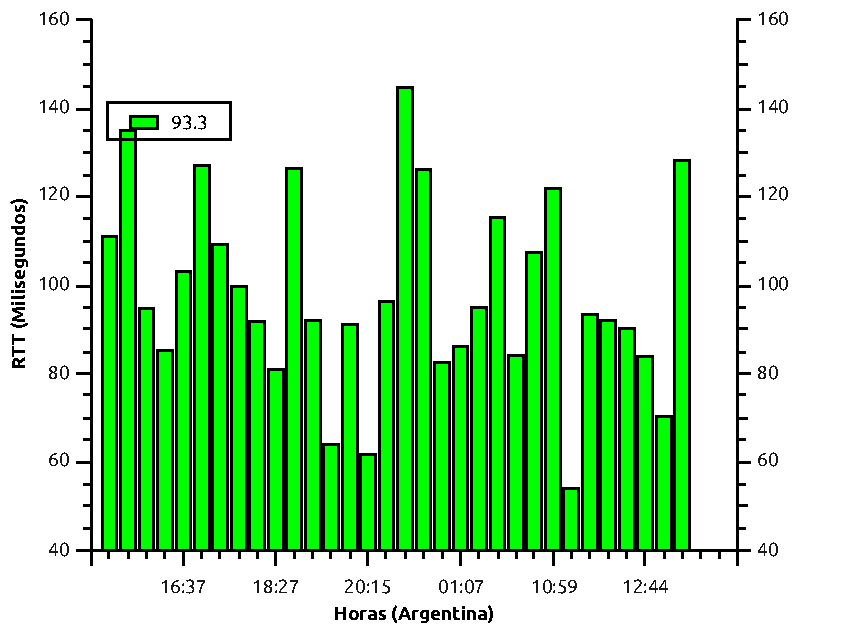
\includegraphics[width=0.9\textwidth]{graficos/rtts_dia_inglaterra.pdf}
    \caption{RTTs medidos a lo largo del dia en un enlace de EEUU a finlandia}
    \label{fig:rtts_ing}
\end{figure}

En el caso de la figura \ref{fig:rtts_ing} se puede ver que, si bien se observan picos en los horarios laborables, durante el resto del día no existe una tendencia o valor representativo. Este es un ejemplo de lo caótico e irregular que puede llegar a ser el tráfico en Internet.